\documentclass[aps,prb,twocolumn,superscriptaddress,floatfix,longbibliography]{revtex4-2}



\usepackage[utf8]{inputenc}
\usepackage[spanish]{babel}
\usepackage{graphicx}
\usepackage{amsmath}
\usepackage{subcaption}
\usepackage{wrapfig} 
\usepackage[export]{adjustbox}

\usepackage{amsmath,amssymb} % math symbols
\usepackage{bm} % bold math font
\usepackage{graphicx} % for figures
\usepackage{comment} % allows block comments
\usepackage{textcomp} % This package is just to give the text quote '
%\usepackage{ulem} % allows strikeout text, e.g. \sout{text}

\usepackage[spanish]{babel}

\usepackage{enumitem}
\setlist{noitemsep,leftmargin=*,topsep=0pt,parsep=0pt}

\usepackage{xcolor} % \textcolor{red}{text} will be red for notes
\definecolor{lightgray}{gray}{0.6}
\definecolor{medgray}{gray}{0.4}

\usepackage{hyperref}
\hypersetup{
colorlinks=true,
urlcolor= blue,
citecolor=blue,
linkcolor= blue,
bookmarks=true,
bookmarksopen=false,
}

% Code to add paragraph numbers and titles
\newif\ifptitle
\newif\ifpnumber
\newcounter{para}
\newcommand\ptitle[1]{\par\refstepcounter{para}
{\ifpnumber{\noindent\textcolor{lightgray}{\textbf{\thepara}}\indent}\fi}
{\ifptitle{\textbf{[{#1}]}}\fi}}
\ptitletrue  % comment this line to hide paragraph titles
\pnumbertrue  % comment this line to hide paragraph numbers

% minimum font size for figures
\newcommand{\minfont}{6}

% Uncomment this line if you prefer your vectors to appear as bold letters.
% By default they will appear with arrows over them.
% \renewcommand{\vec}[1]{\bm{#1}}

%Cambiar Cuadros por Tablas y lista de...
%\renewcommand{\listtablename}{Índice de tablas}
\renewcommand{\tablename}{Tabla}
\renewcommand{\date}{Fecha}

\usepackage[bottom]{footmisc} %para que las notas al pie aparezcan en la misma página



\begin{comment}

%Comandos de interés:

* Para ordenar el documento:
\section{Introducción}
\section{\label{sec:Formatting}Formatting} %label para luego hacer referencia a esa sección

\ptitle{Start writing while you experiment} %pone nombre y título al documento dependiendo de si en el header están los comandos \ptitletrue y \pnumbertrue

* Ecuaciones:
\begin{equation}
a^2+b^2=c^2 \,.
\label{eqn:Pythagoras}
\end{equation}

* Conjunto de ecuaciones:
\begin{eqnarray}
\label{eqn:diagonal}
\nonumber d & = & \sqrt{a^2 + b^2 + c^2} \\
& = & \sqrt{3^2+4^2+12^2} = 13
\end{eqnarray}

* Para hacer items / enumerar:
\begin{enumerate}
  \item
\end{enumerate}

\begin{itemize}
  \item
\end{itemize}

* Figuras:
\begin{figure}[h]
    \includegraphics[clip=true,width=\columnwidth]{pixel-compare}
    \caption{}
     \label{fig:pixels}
\end{figure}

* Conjunto de figuras:
(no recuerdo)


* Para hacer referencias a fórmulas, tablas, secciones, ... dentro del documento:
\ref{tab:spacing}

* Para citar
Elementos de .bib
\cite{WhitesidesAdvMat2004}
url
\url{http://www.mendeley.com/}\\

* Agradecimientos:
\begin{acknowledgments}
We acknowledge advice from Jessie Zhang and Harry Pirie to produce Fig.\ \ref{fig:pixels}.
\end{acknowledgments}

* Apéndice:
\appendix
\section{\label{app:Mendeley}Mendeley}

* Bibliografía:
\bibliography{Hoffman-example-paper}

\end{comment}

\begin{comment}

Plots y tablas en orden:

* Figura de los cilindros con los PT100, la resistencia de referencia, la fuente, el multímetro y la computadora simbolizando el software de adquisisción de datos.
* Figura de los cilindros con la lampartira, la fuente que le da tensión y el multímetro para medir esa tensión

* Tabla de dimensiones de los cilindros
(la copio de prácticos anteriores)

* Figura del equipo de algto vacío (bomba mecánica, difusora, tubos, bridas, cámara, 3 cilindros...)
* Figura sobre cómo determinar epsilon (pirómetro, termocupla apoyados sobre cilindro exterior sin vacío)

PLOT PPAL:
* T vs t mostrando un gráfico lindo donde se vea bien el transitorio y el estacionario

SUBPLOTS:
* T vs t mostrando qué pasa si hay un cortocircuito interno que hace que la lámpara no prenda (se ven T bajas)
* T vs t mostrando qué pasa si no ponemos el telgopor
* T vs t mostrando qué pasa si falla el vacío
* T vs t mostrando qué pasa en el cilindro externo cuando agregamos N2
* T vs t mostrando qué pasa cuando cambiamos la potencia de la lamparita sobre la marcha



Determinación del producto de ctes
* T vs P recta para calcular la pendiente relacionada con el producto de constantes

Determinación de epsilon
* Gráfico Epsilon vs P

Bibliografía:
* Agregar referencia a la tabla de calibración R vs T
* Agregar referencia a que sacamos los datos de las áreas de un práctico de años anteriores

\end{comment}



\begin{document}

% Allows to rewrite the same title in the supplement
\newcommand{\mytitle}{TP 01 - Diferencias finitas - EDO }

\title{\mytitle}

\author{Pablo Chehade \\
    \small \textit{pablo.chehade@ib.edu.ar} \\
    \small \textit{Física computacional, Instituto Balseiro, CNEA-UNCuyo, Bariloche, Argentina} \\}


\maketitle

\section{Ejercicio 3}
Se parte del siguiente modelo de un sistema de reacciones químicas
\begin{equation}
\frac{dx}{dt} = a - (b+1) x + x^2 y = f(x,y(t))
\label{eq:1erEDO}
\end{equation}

\begin{equation}
\frac{dy}{dt} = b x - x^2 y = g(x(t),y)
\label{eq:2daEDO}
\end{equation}

Aplicando el método RK4 a la primer ecuación diferencial se obtiene
\[x_{j+1} \approx x_j + \frac{h}{6} (k_{1x} + 2k_{2x} + 2k_{3x} + k_{4x})\]
donde
\[k_{1x} = f(x_j, y(t_j)\]
\[k_{2x} = f(x_j + \frac{h}{2} k_{1x},y(t_j + \frac{h}{2})) \]
\[k_{3x} = f(x_j + \frac{h}{2} k_{2x},y(t_j + \frac{h}{2}))\]
\[k_{4x} = f(x_j + h k_{3x},y(t_j + h))\]

Se observa que para calcular $x_{j+1}$ se necesita información sobre $y$. Lo mimso ocurre con $y_{j+1}$ respecto de $x$. Este procedimiento recursivo no  permite avanzar a menos que se realicen algunas consideraciones. En primer lugar, es claro que  $y(t_j) = y_j$. En segundo lugar, dado que no se tiene información sobre $y(t_j + \frac{h}{2})$, se podría aproximar por el promedio $y(t_j + \frac{h}{2}) \approx \frac{y_{j+1} + y_j}{2}$ donde $y_{j+1} = y(t_j+h)$. Tampoco se tiene información de este último pero se puede aproximar por el método de Euler $y_{j+1} \approx y_j + h g(x_j,y_j)$ aprovechando la segunda ecuación diferencial \ref{eq:2daEDO}.
En base a esto
\[k_{1x} = f(x_j, y(t_j))\]
\[k_{2x} = f(x_j + \frac{h}{2} k_{1x},y_j + \frac{h}{2} g(x_j,y_j))\]
\[k_{3x} = f(x_j + \frac{h}{2} k_{2x},y_j + \frac{h}{2} g(x_j,y_j))\]
\[k_{4x} = f(x_j + h k_{3x},y_j + h g(x_j,y_j))\]

El procedimiento para la segunda ecuación diferencial es análogo
\[y_{j+1} \approx y_j + \frac{h}{6} (k_{1y} + 2k_{2y} + 2k_{3y} + k_{4y})\]
donde $k_{yi}$ se definen de manera similar a los $k_{xi}$, $i = $ 1, 2, 3, 4. Cabe aclarar que el método descripto anteriormente es una variante de RK4 dadas las aproximaciones realizadas. Establecido esto, lo único que falta es definir hasta qué momento se realizarán las iteraciones. El criterio considerado consta del cumplimiento de una de dos condiciones:
\begin{enumerate}
    \item Los errores en $x$ e $y$ estimados como la diferencia entre un valor y el siguiente: $\Delta x = |x_{j+1} - x_j|$ y $\Delta y = |y_{j+1} - y_j|$, son menores a una toleracia global 'tolg' en ambos casos.
    \item Se llega a un número máximo de iteraciones 'jmax'.
\end{enumerate}
Es claro que si se cumple (1) para tolg 'tan pequeño como se quiera' se está en presencia de un equilibrio estable. Mientras que si se cumple (2) para jmax 'tan grande como se quiera', de uno inestable.

\subsection{Inciso a}
Se aplicó el método para $a = b = 1$ empleando distintos pasos. Se obtuvieron los resultados graficados en la figura \ref{fig:3_a}. La curva con $h = 0.001$ se usa como referente de la solución. Como el paso es pequeño (en concreto, menor que los demás), el método asegura que se trata de una mejor aproximación que las demás.

\begin{figure}[h]
    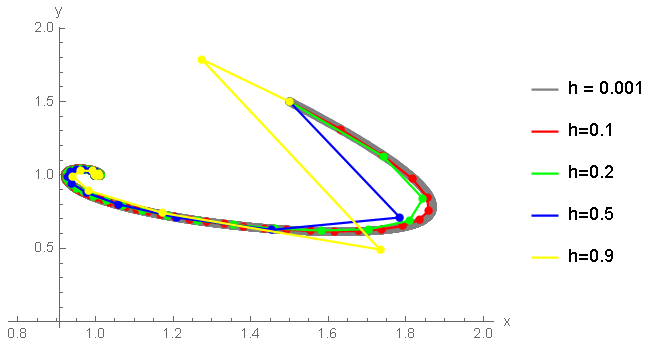
\includegraphics[clip=true,width=\columnwidth]{3_a.png}
    \caption{Soluciones numéricas con distintos pasos $h$ para $a = b = 1$.}
     \label{fig:3_a}
\end{figure}

Por un lado se observa que las soluciones numéricas convergen al equilibrio $x_0^* = 1$, $y_0^* = 1$ para los casos $h = 0.1, 0.2, 0.5$ y $0.9$. ¿Cómo se asegura que se llegó al equilibrio? Las iteraciones se detienen porque se cumplió la condición de tolerancia global, no llegando a la cantidad máxima de iteraciones permitidas. Por otro lado, para el caso $h = 1.0$ el programa registra un overflow por lo que se interpreta que no converge (o bien hay algún problema en el código). En definitiva, se prueba que el método converge aún para pasos 'grandes' con una cota superior que en este caso sería $h = 1.0$.

\subsection{Inciso b}


Se aplicó el método para $a = 1$, $b = 3$ con distintas condiciones iniciales como se puede observar en las figuras \ref{fig:3_b_x0_1} y \ref{fig:3_b_x0_3}. Las condiciones iniciales corresponden a un punto fuera del ciclo y cerca de las condiciones de equilibrio $x_0^* = 1$, $y_0^* = 3$. En ambos casos la solución tiende a un ciclo límite. En la figura \ref{fig:3_b_x0_3} es notorio que la solución es inestable: incluso cerca de las condiciones de equilibrio el sistema evoluciona alejándose del mismo. ¿Cómo se asegura la inestabilidad? Las iteraciones se detienen porque se cumple el número máximo de iteraciones y no por la condición de tolerancia global. 


\begin{figure}[h]
    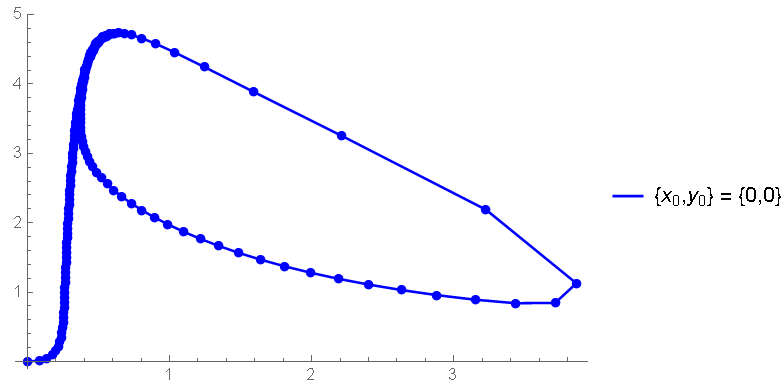
\includegraphics[clip=true,width=\columnwidth]{3_b_x0_1.png}
    \caption{Solución numérica con paso $h = 0.1$ para $a = 1$, $b = 3$ con condición inicial fuera del ciclo.}
     \label{fig:3_b_x0_1}
\end{figure}

\begin{figure}[h]
    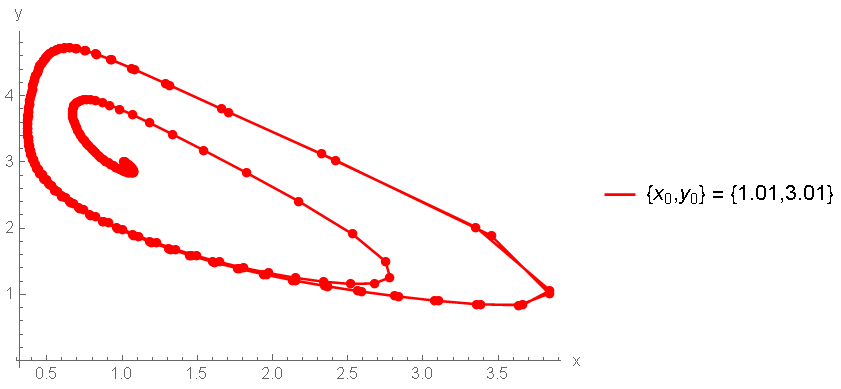
\includegraphics[clip=true,width=\columnwidth]{3_b_x0_3.png}
    \caption{Solución numérica con paso $h = 0.1$ para $a = 1$, $b = 3$ con condición inicial cercana a la condición de equilibrio.}
     \label{fig:3_b_x0_3}
\end{figure}

Además, se aplicó el método para distintos pasos $h = 0.1, 0.15$ como se observa en la figura \ref{fig:3_b_h}. Ocurre que para el caso $h = 0.15$ y pasos mayores la solución numérica diverge.


\begin{figure}[h]
    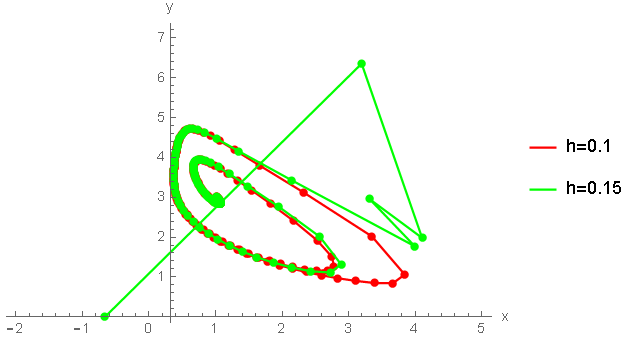
\includegraphics[clip=true,width=\columnwidth]{3_b_h.png}
    \caption{Solución numérica con distintos pasos para $a = 1$, $b = 3$.}
     \label{fig:3_b_h}
\end{figure}


\section{Ejercicio 4}

Se implementa un paso adaptativo para el caso $a = 1$, $b =3$ bajo la estrategia presentada en la siguiente tabla.

\begin{table}[h]
\begin{tabular}{l|c|c|c|}
\cline{2-4}
\multicolumn{1}{c|}{} &
  \multicolumn{1}{l|}{$\Delta x < \epsilon /2$} &
  \multicolumn{1}{l|}{$\epsilon / 2< \Delta x < \epsilon$} &
  \multicolumn{1}{l|}{$\Delta x > \epsilon$} \\ \hline
\multicolumn{1}{|l|}{$\Delta y < \epsilon /2$} &
  \begin{tabular}[c]{@{}c@{}}acepto\\ $h \rightarrow 1.5 h$\end{tabular} &
  \begin{tabular}[c]{@{}c@{}}acepto\\ $h \rightarrow h$\end{tabular} &
  \begin{tabular}[c]{@{}c@{}}rechazo\\ $h \rightarrow 1.5 h$\end{tabular} \\ \hline
\multicolumn{1}{|l|}{$\epsilon / 2< \Delta y < \epsilon$} &
  \begin{tabular}[c]{@{}c@{}}acepto\\ $h \rightarrow h$\end{tabular} &
  \begin{tabular}[c]{@{}c@{}}acepto\\ $h \rightarrow h$\end{tabular} &
  \begin{tabular}[c]{@{}c@{}}rechazo\\ $h \rightarrow 1.5 h$\end{tabular} \\ \hline
\multicolumn{1}{|l|}{$\Delta y > \epsilon$} &
  \begin{tabular}[c]{@{}c@{}}rechazo\\ $h \rightarrow 1.5 h$\end{tabular} &
  \begin{tabular}[c]{@{}c@{}}rechazo\\ $h \rightarrow 1.5 h$\end{tabular} &
  \begin{tabular}[c]{@{}c@{}}rechazo\\ $h \rightarrow 1.5 h$\end{tabular} \\ \hline
\end{tabular}

\end{table}


Inicialmente se considéró $\epsilon = 10^{-2}$ y se obtuvieron las soluciones numéricas $x(t)$ e $y(t)$ graficadas en la figura \ref{fig:4_xy_2}. Además, en la figura \ref{fig:4_fases_2} los mismos datos se grafican en el espacio de fases. Se empleó una condición inical cercana al ciclo de modo de identificar fácilmente cuando se cumple un período, es decir, una revolución en el ciclo límite. Se observa que a pesar de que las soluciones varían rápidamente en distintas regiones, el paso adaptativo es capaz de adaptarse. Esto se observa en la figura \ref{fig:4_h_2} donde se grafica el paso $h$ en función del tiempo $t$ y, simultáneamente, el módulo $\sqrt{x^2 + y^2}$ en función de $t$. Este último se puede utilizar para observar cómo varían $x(t)$ e $y(t)$. Cuando el modulo se mantiene constante, h crece porque los errores la diferencia entre un valor $j$ y el siguiente $j+1$ es pequeña o se mantiene porque se está en el rango $[\epsilon / 2, \epsilon]$. En cambio, cuando el módulo varía drásticamente, h decrece porque se está en la condición en la que el error es mayor a la tolerancia.

\begin{figure}[]
    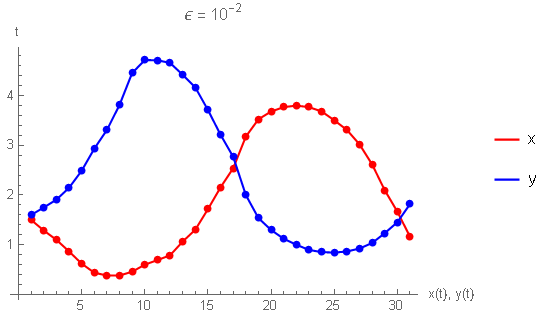
\includegraphics[clip=true,width=0.8\columnwidth]{4_xy_2.png}
    \caption{Solución numérica $x(t)$ e $y(t)$ con paso adaptativo para $a = 1$, $b = 3$ con tolerancia $\epsilon = 10^{-2}$ y condición inicial cercana al ciclo límite.}
     \label{fig:4_xy_2}
\end{figure}

\begin{figure}[]
    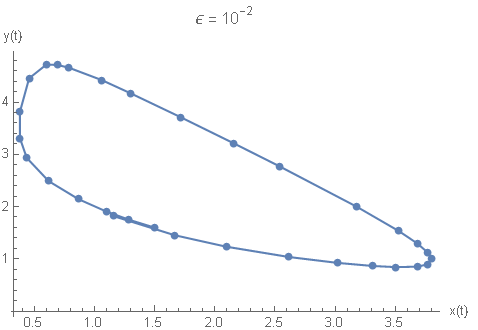
\includegraphics[clip=true,width=0.8\columnwidth]{4_fases_2.png}
    \caption{Solución numérica en el espacio de fases con paso adaptativo para $a = 1$, $b = 3$ con tolerancia $\epsilon = 10^{-2}$ y condición inicial cercana al ciclo límite.}
     \label{fig:4_fases_2}
\end{figure}

\begin{figure}[]
    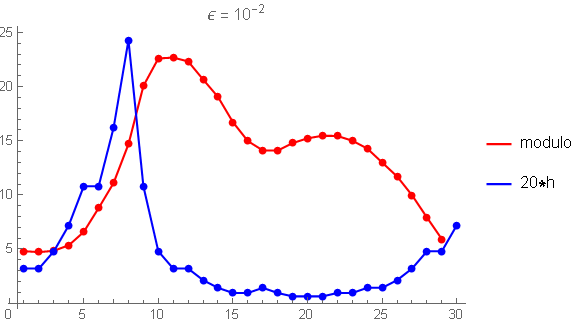
\includegraphics[clip=true,width=0.8\columnwidth]{4_h_2.png}
    \caption{$h$ y módulo en función de $t$ para la solución numérica con paso adaptativo para $a = 1$, $b = 3$ con condición inicial cercana al ciclo límite.}
     \label{fig:4_h_2}
\end{figure}


En un período el algoritmo de paso adaptativo realizó alrededor de 30 pasos. Mientras que, implementando el algoritmo del ejercicio anterior bajo la condición de que el máximo error cometido sea menor que la tolerancia, se necesitó un paso de $h = 0.001$ y $7200$ pasos aproximadamente. Esto implica que el paso adaptativo es más eficiente que la estrategia empleada en el ejercicio anterior y es más notorio a menor tolerancia. Esto último se debe a que si en cambio se emplea como tolerancia $\epsilon = 10^{-5}$, se obtienen las soluciones numéricas graficadas en la figura \ref{fig:4_xy_5} en función del $t$ y en la figura \ref{fig:4_fases_5} en el espacio de fases. En un período el algoritmo de paso adaptativo realizó alrededor de 280 pasos. Mientras que, implementando el algoritmo del ejercicio anterior bajo la condición de que el máximo error cometido sea menor que la tolerancia, se necesitó un paso de $h = 0.00001$ y más de $500000$ pasos aproximadamente. Además, para esta nueva tolerancia no se encontraron diferencias respecto al análisis realizado en base a la figura \ref{fig:4_h_2}.

\begin{figure}[]
    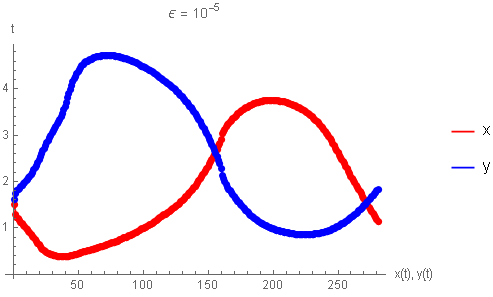
\includegraphics[clip=true,width=0.8\columnwidth]{4_xy_5.png}
    \caption{Solución numérica $x(t)$ e $y(t)$ con paso adaptativo para $a = 1$, $b = 3$ con tolerancia $\epsilon = 10^{-5}$ y condición inicial cercana al ciclo límite.}
     \label{fig:4_xy_5}
\end{figure}

\begin{figure}[]
    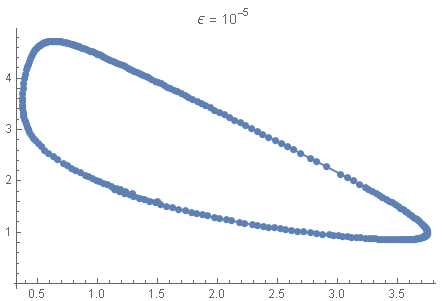
\includegraphics[clip=true,width=0.8\columnwidth]{4_fases_5.png}
    \caption{Solución numérica en el espacio de fases con paso adaptativo para $a = 1$, $b = 3$ con tolerancia $\epsilon = 10^{-5}$ y condición inicial cercana al ciclo límite.}
     \label{fig:4_fases_5}
\end{figure}


\bibliography{Radiacion_de_cuerpo_negro}

\end{document}

